\documentclass[aspectratio=43,t]{beamer}  
\usepackage{setspace}
\linespread{1.3}
\usepackage{amssymb, amsmath, amsthm}
\usepackage{appendixnumberbeamer}
\usepackage{transparent,booktabs}
\usepackage{pgfpages}
\usepackage{xcolor}
\usepackage{verbatim}

\usetheme{metropolis}
\setbeamersize{text margin left=0.7cm, text margin right=0.7cm}
%\setbeamertemplate{footline}{} 


\setbeamercolor{background canvas}{bg=white}
\definecolor{UBCblue}{rgb}{0.04706, 0.13725, 0.26667} % UBC Blue (primary)
\definecolor{UBCgrey}{rgb}{0.3686, 0.5255, 0.6235} % UBC Grey (secondary)

\setbeamercolor{palette primary}{bg=UBCblue,fg=white}
\setbeamercolor{palette secondary}{bg=UBCblue,fg=white}
\setbeamercolor{palette tertiary}{bg=UBCblue,fg=white}
\setbeamercolor{palette quaternary}{bg=UBCblue,fg=white}
\setbeamercolor{structure}{fg=UBCblue} % itemize, enumerate, etc
\setbeamercolor{section in toc}{fg=UBCblue} % TOC sections
\setbeamercolor{subsection in head/foot}{bg=UBCgrey,fg=white}
\setbeamercolor{progress bar}{fg=UBCblue,bg=UBCgrey}
\setbeamercolor{alerted text}{fg=UBCblue}

%gets rid of navigation symbols
\setbeamertemplate{navigation symbols}{}

%\setbeameroption{show notes}
%\setbeameroption{show only notes}
%\setbeameroption{hide notes}
%\setbeameroption{show notes on second screen}

%%%%%%%%%%%%%%%%%%%%%%%%%%%%%%%%%%%%%%%%%%%%%%
\title[TALK]{\Large{Proxyvariable, målefejl og manglende data}}
\subtitle{Økonometri A}
\author{Bertel Schjerning}
\date{}

%%%%%%%%%%%%%%%%%%%%%%%%%%%%%%%%%%%%%%%%%%%%%%
\begin{document} 
\maketitle
%%%%%%%%%%%%%%%%%%%%%%%%%%%%%%%%%%%%%%%%%%%%%%

%%%%%%%%%%%%%%%%%%%%%%%%%%%%%%%%%%%%%%%%%%%%%%
\begin{frame}
\frametitle{Program}
	\tableofcontents
\end{frame}
%%%%%%%%%%%%%%%%%%%%%%%%%%%%%%%%%%%%%%%%%%%%%%

%%%%%%%%%%%%%%%%%%%%%%%%%%%%%%%%%%%%%%%%%%%%%%
\begin{frame}
\frametitle{Motivation}

	Nogle gange har vi ikke præcis de variable, vi kunne ønske os.
	
	Fx hvis vi
	\begin{itemize}
	\item Skal estimere effekten af skat på arbejdsudbuddet, skal vi kende folks marginalskat. 
	\item Ønsker at kontrollere for ``evne'' i regressionen af løn på uddannelse.
	\item Bruger surveydata, hvor folk selv har skullet oplyse formue mv.
	\end{itemize}
		
\end{frame}

%%%%%%%%%%%%%%%%%%%%%%%%%%%%%%%%%%%%%%%%%%%%%%

%%%%%%%%%%%%%%%%%%%%%%%%%%%%%%%%%%%%%%%%%%%%%%
\begin{frame}
\frametitle{Motivation}

	Overordnet skelner vi mellem:
	\begin{itemize}

\item \textbf{Proxyvariable}: Proxy for en uobserveret variabel, som \textbf{ikke har en præcis kvantitativ fortolkning}.
\smallskip

\begin{itemize}
\item Fx helbred eller evner, som kan være svære at kvantificere.

\item Vi er ofte ikke interesserede i effekten af variablen, men ønsker at kontrollere for den.
\end{itemize}
\medskip
	
\item \textbf{Målefejl}: Variable opgjort med målefejl, som har en \textbf{præcis kvantitativ fortolkning}.
\smallskip

\begin{itemize}
\item Fx har forbrug en præcis betydning, men selvrapporterede
forbrugsudgifter kan være målt med fejl.
\item Folk husker forkert eller har glemt indkøb.

\item Vi er ofte interesserede i parameteren til variablen.

\end{itemize}

\end{itemize}

\end{frame}
	
%%%%%%%%%%%%%%%%%%%%%%%%%%%%%%%%%%%%%%%%%%%%%%


\section[Proxyvariable]{Proxyvariable (W9.2)}


%%%%%%%%%%%%%%%%%%%%%%%%%%%%%%%%%%%%%%%%%%%%%%
\begin{frame}
\frametitle{Proxyvariable}

	Antag at den sande model er givet ved
	\begin{equation}
	y = \beta_0 + \beta_1 x_1 + \beta_2 x^*_2 + u
	\end{equation}
	hvor vi er interesserede i $\beta_1$.
	$x^*_2$ er således kun med i modellen for at den opfylder MLR.1-MLR.4. Det antager vi her.
	
	\textbf{$x^*_2$ er dog uobserveret.}
	
	I stedet observerer vi en proxy $x_2$, som er korreleret med $x^*_2$:
	\begin{equation}
	x^*_2 = \delta_0 + \delta_1 x_2 + v, \text{ med } \delta_1 \neq 0
	\end{equation}
	Spørgsmålet er nu, om vi kan få et middelret estimat ved at inkludere $x_2$ i stedet for $x^*_2$.
		
\end{frame}

%%%%%%%%%%%%%%%%%%%%%%%%%%%%%%%%%%%%%%%%%%%%%%

%%%%%%%%%%%%%%%%%%%%%%%%%%%%%%%%%%%%%%%%%%%%%%
\begin{frame}
\frametitle{Proxyvariable}
	
	Hvis vi indsætter ligning (2) i ligning (1) får vi
	\begin{align*}
	y &=& \beta_0                         &+& \beta_1 x_1 &+& \beta_2 (\delta_0 + \delta_1 x_2 + v) &+& u \\
	  &=& \beta_0+ \beta_2 \cdot \delta_0 &+& \beta_1 x_1 &+& \beta_2 \delta_1 x_2                  &+& u + \beta_2v \\
	  &=& \tilde{\beta}_0                 &+& \beta_1 x_1 &+& \tilde{\beta}_2 x_2                   &+& e
	\end{align*}
	Vi kan få et middelret estimat af $\beta_1$, hvis det nye fejlled opfylder MLR.4:
	\begin{align*}
	E(e|x_1,x_2)&=E(u+\beta_2v|x_1,x_2)=0.
	\end{align*}	
	Et tilstrækkeligt, men ikke automatisk opfyldt, sæt betingelser er
	\begin{equation*}
	E(u|x_1,x_2)=0
	\quad\text{og}\quad
	E(v|x_1,x_2)=0.
	\end{equation*}
\end{frame}

%%%%%%%%%%%%%%%%%%%%%%%%%%%%%%%%%%%%%%%%%%%%%%

%%%%%%%%%%%%%%%%%%%%%%%%%%%%%%%%%%%%%%%%%%%%%%
\begin{frame}
\frametitle{Proxyvariable: Eksempel}
	
	Antag at MLR.1-MLR.4 er opfyldt for den følgende model
	\begin{equation}
		\log(\text{løn}) = \beta_0 + \beta_1 uddannelse + \beta_2 evner + u
	\end{equation}
	Vi observerer ikke folks sande evner, men vi kan observere
	\begin{equation}
		evner = \delta_0 + \delta_1 IQ + v
	\end{equation}
	OLS-estimation af (3) med IQ som proxy for evner er middelret, hvis
	\begin{equation}
		E(u+\beta_2v|uddannelse,IQ) = 0.
	\end{equation}	
	\textbf{Er det en rimelig antagelse?}

	Blandt personer med samme IQ kan uddannelse stadig hænge sammen med fx motivation, selvdisciplin og familiebaggrund.
	
\end{frame}

%%%%%%%%%%%%%%%%%%%%%%%%%%%%%%%%%%%%%%%%%%%%%%

%%%%%%%%%%%%%%%%%%%%%%%%%%%%%%%%%%%%%%%%%%%%%%
\begin{frame}
\frametitle{Bias uden proxy}
	
	Vi kan sammenligne den asymptotiske bias ved helt at undlade $x^*_2$ og ved at anvende en proxy.
	
	Bias ved undladelse
	\begin{equation*}
	p\text{lim } \hat{\beta}_1^{u} - \beta_1 
	= \beta_2 \frac{\text{cov}(x_1,x^*_2)}{\text{var}(x_1)} 
	= \beta_2 \frac{\delta_1\text{cov}(x_1, x_2)+\text{cov}(x_1,v)}{\text{var}(x_1)} 
	\end{equation*}	
	Uden proxy ligger hele $x_2^*$ i fejlleddet. Både den del, som $x_2$ opfanger, og den resterende del $v$ kan derfor skabe bias.

\end{frame}

%%%%%%%%%%%%%%%%%%%%%%%%%%%%%%%%%%%%%%%%%%%%%%

%%%%%%%%%%%%%%%%%%%%%%%%%%%%%%%%%%%%%%%%%%%%%%
\begin{frame}
\frametitle{Bias med proxy}

	Lad $r_1$ være residualet fra populationsprojektionen af $x_1$ på et konstantled og $x_2$. FWL giver
	\begin{equation*}
	p\text{lim } \hat{\beta}_1^{m} - \beta_1 
	= \frac{\text{cov}(r_1,u+\beta_2v)}{\text{var}(r_1)}.
	\end{equation*}		
	Hvis $\text{cov}(r_1,u)=0$, kommer den resterende bias fra den del $v$, som proxyen ikke opfanger:
	\begin{equation*}
	p\text{lim } \hat{\beta}_1^{m} - \beta_1
	=\beta_2\frac{\text{cov}(r_1,v)}{\text{var}(r_1)}.
	\end{equation*}
	En proxy kan derfor reducere bias, men det er ikke garanteret.
	
\end{frame}

%%%%%%%%%%%%%%%%%%%%%%%%%%%%%%%%%%%%%%%%%%%%%%


\section[Målefejl]{Målefejl (W9.4)}

\subsection{Målefejl i den afhængige variabel}

%%%%%%%%%%%%%%%%%%%%%%%%%%%%%%%%%%%%%%%%%%%%%%

%%%%%%%%%%%%%%%%%%%%%%%%%%%%%%%%%%%%%%%%%%%%%%
\begin{frame}
\frametitle{Målefejl i den afhængige variabel}
	
	Antag at vi har følgende model
	\begin{equation*}
	y^{*}=\beta _{0}+\beta _{1}x_{1}+\beta _{2}x_{2}+...+\beta _{k}x_{k}+u,
	\end{equation*}
	hvor MLR.1-MLR.4 er opfyldt.

	\begin{itemize}
	\item $y^{*}$ er \textbf{uobserveret}.
	
	\item I stedet observerer vi $y = y^{*}+e$

	\item $e$ er en målefejl: $e = y - y^{*}$.
	\end{itemize}
	
	\textbf{Hvad er konsekvensen ved at anvende $y$ i stedet for $y^{*}$?}
	
	Estimationsmodel
	\begin{equation*}
	y=y^{\ast }+e =\beta _{0}+\beta _{1}x_{1}+\beta _{2}x_{2}+...+\beta_{k}x_{k}+u+e
	\end{equation*}

\end{frame}

%%%%%%%%%%%%%%%%%%%%%%%%%%%%%%%%%%%%%%%%%%%%%%

%%%%%%%%%%%%%%%%%%%%%%%%%%%%%%%%%%%%%%%%%%%%%%
\begin{frame}
\frametitle{Målefejl i den afhængige variabel}
	
	Vil OLS-estimatoren være middelret og konsistent?

	Det kræver, at der for det nye fejlled $u+e$ gælder: 
	\begin{align*}
	E(u+e|X) &= E(u|X)+E(e|X) \\
			   &= 0+E(e|X)=0.
	\end{align*}
	\begin{itemize}
	\item Det er nok, at $E(e|X)$ er konstant: Konstantleddet absorberer middelværdien.

	\item Antagelsen $E(e|X)=0$ gælder fx, hvis $e$ er uafhængig af $x_{1},x_{2},\ldots,x_{k}$.

	\item Så vil \textbf{OLS-estimatoren} i en model med målefejl i
	den afhængige variabel stadig være \textbf{middelret og konsistent}.
\end{itemize}

\end{frame}

%%%%%%%%%%%%%%%%%%%%%%%%%%%%%%%%%%%%%%%%%%%%%%

%%%%%%%%%%%%%%%%%%%%%%%%%%%%%%%%%%%%%%%%%%%%%%
\begin{frame}
\frametitle{Målefejl i den afhængige variabel}
	
	Er $E(e|X)=0$ en realistisk antagelse?
	
	\begin{itemize}
		\item Ofte ja.
		\medskip
		\item Men ikke altid.
		\medskip
		\item Hvis rige underrapporterer deres indkomst/formue.
	\end{itemize}

\end{frame}

%%%%%%%%%%%%%%%%%%%%%%%%%%%%%%%%%%%%%%%%%%%%%%

%%%%%%%%%%%%%%%%%%%%%%%%%%%%%%%%%%%%%%%%%%%%%%
\begin{frame}
\frametitle{Målefejl i den afhængige variabel}
	
	Hvad med variansen på OLS-estimatoren?
	
	\begin{itemize}
	\item Hvis $u$ og $e$ er ukorrelerede og homoskedastiske, får vi
	\begin{equation*}
	\text{var}(u+e|X) = \sigma_{u}^{2}+\sigma_{e}^{2} > \sigma_{u}^{2}.
	\end{equation*}
	\end{itemize}
	Dvs. større varians af fejlleddet, hvis der er målefejl i den afhængige variabel.

	$\rightarrow$ Større varians på parameterestimatoren $\text{var}(\hat{\beta}_{j}|X)$ og mindre præcision.

\end{frame}

%%%%%%%%%%%%%%%%%%%%%%%%%%%%%%%%%%%%%%%%%%%%%%

%%%%%%%%%%%%%%%%%%%%%%%%%%%%%%%%%%%%%%%%%%%%%%
\begin{frame}
\frametitle{Multiplikative målefejl}

	 Nogle gange giver det mere mening at antage, at målefejlen er multiplikativ.
	\begin{itemize}
	\item Fx hvis størrelsen af målefejlene er proportional med $y$-variablen.

	\item Afhængig variabel:
	\begin{equation*}
	y=y^{*}\cdot a, \quad a>0
	\end{equation*}
	\end{itemize}	
	Logaritmen gør målefejlen additiv:
	\begin{align*}
	\log (y) &= \log (y^{*}) + \log(a) \\ 
		      &= \log (y^{*}) + e,  
	\end{align*}
	hvor $e = \log (a)$.

	Dvs. vi er tilbage i setuppet fra før. Men logaritmen løser kun problemet, hvis $E(\log(a)|X)$ er konstant.

	%Multiplikative m{\aa}lefejl kan også optr{\ae}de for forklarende variable. Samme løsning.
	
\end{frame}

%%%%%%%%%%%%%%%%%%%%%%%%%%%%%%%%%%%%%%%%%%%%%%


\subsection{Målefejl i forklarende variable}


%%%%%%%%%%%%%%%%%%%%%%%%%%%%%%%%%%%%%%%%%%%%%%
\begin{frame}
\frametitle{Målefejl i forklarende variable}

	Vi betragter igen den sande model
	\begin{equation*}
	y=\beta_{0}+\beta_{1}x^{*}+u,
	\end{equation*}
	hvor MLR.1-MLR.4 er opfyldt.
	\begin{itemize}
	\item $x^{*}$ er ikke observeret.
	\item Forholdet mellem $x^*$ og det observerede $x$ bestemmer konsekvensen.
	\end{itemize}
	
	To tilfælde:
	\begin{enumerate}
	\item $x^*=x+e$ og $E(e|x)=0$: Berkson-målefejl.
	
	\item $x=x^*+e$ og $\text{cov}(e,x^{*})=0$: Klassisk målefejl.
	\end{enumerate}

\end{frame}

%%%%%%%%%%%%%%%%%%%%%%%%%%%%%%%%%%%%%%%%%%%%%%

%%%%%%%%%%%%%%%%%%%%%%%%%%%%%%%%%%%%%%%%%%%%%%
\begin{frame}
\frametitle{Tilfælde 1: Berkson-målefejl}

	Indsæt $x^{*}=x+e$ i modellen:
	\begin{align*}
	y &=\beta_{0} + \beta_{1}x^{*}	&+u 		\\
	  &=\beta_{0} + \beta_{1}(x+e)	&+u 		\\
	  &=\beta_{0} + \beta_{1}x      &+u +\beta_{1}e.
	\end{align*}
	Hvis $E(u|x)=0$ og $E(e|x)=0$, er det nye fejlled middelret:
	\begin{align*}
	E(u+\beta_1e|x)=0.
	\end{align*}
	Derfor er OLS middelret og konsistent. Berkson-målefejl opstår fx, når alle i en gruppe tildeles samme mål, mens deres sande værdier varierer omkring gruppemålet.

\end{frame}

%%%%%%%%%%%%%%%%%%%%%%%%%%%%%%%%%%%%%%%%%%%%%%

%%%%%%%%%%%%%%%%%%%%%%%%%%%%%%%%%%%%%%%%%%%%%%
\begin{frame}
\frametitle{Tilfælde 2: Klassisk målefejl}

	Indsæt igen $x^{*}=x-e$ i modellen
	\begin{equation*}
	y=\beta_{0}+\beta_{1}x+u-\beta_{1}e.
	\end{equation*}
	Antag $\text{cov}(u,x^*)=\text{cov}(u,e)=\text{cov}(e,x^*)=0$. For det nye fejlled gælder:
	\begin{align*}
	\text{cov}(u-\beta_1e,x)
	&=\text{cov}(u-\beta_1e,x^*+e)\\
	&=-\beta_1\text{var}(e)=-\beta_1\sigma_e^2.
	\end{align*}
	Det observerede $x$ er derfor korreleret med det nye fejlled.

\end{frame}

%%%%%%%%%%%%%%%%%%%%%%%%%%%%%%%%%%%%%%%%%%%%%%

%%%%%%%%%%%%%%%%%%%%%%%%%%%%%%%%%%%%%%%%%%%%%%
\begin{frame}
\frametitle{Tilfælde 2: Klassisk målefejl}

	Den asymptotiske bias af $\hat{\beta_1}$ er nu
	\begin{align*}
	p\lim \hat{\beta}_{1}-\beta _{1} &= \frac{\text{cov}(u-\beta _{1}e,x)}{\text{var}(x)} \\
											 &= -\beta_{1}\frac{\sigma_e^2}{var(x^{*} + e)} \\
											 &= -\beta_{1}\frac{\sigma_e^2}{\sigma_{x^*}^2+\sigma_e^2}
	\end{align*}
	Dermed er sandsynlighedsgrænsen
	\begin{equation*}
	p\lim \hat{\beta}_{1}
	=\beta_1\frac{\sigma_{x^*}^2}{\sigma_{x^*}^2+\sigma_e^2}.
	\end{equation*}

\end{frame}

%%%%%%%%%%%%%%%%%%%%%%%%%%%%%%%%%%%%%%%%%%%%%%

%%%%%%%%%%%%%%%%%%%%%%%%%%%%%%%%%%%%%%%%%%%%%%
\begin{frame}
\frametitle{Tilfælde 2: Klassisk målefejl}

\textbf{Konklusion:} OLS-estimatoren er inkonsistent og attenueret mod nul, da
	\begin{equation*}
	0<\frac{\sigma _{x^{*}}^{2}}{\sigma_{x^{*}}^{2}+\sigma_{e}^{2}}<1
	\end{equation*}
\vspace{-0.5cm}
\begin{itemize}
\item Hvis $\beta_{1}>0$ så er $p\lim \hat{\beta}_{1}<\beta_{1}$

\item Hvis $\beta_{1}<0$ så er $p\lim \hat{\beta}_{1}>\beta _{1}$

\item Jo større målefejlsvariansen er, jo større er den asymptotiske bias. %signal-to-noise ratio.
\end{itemize}
Dette kalder vi typisk for \textbf{attenuation bias}.

For flere forklarende variable bliver det mere kompliceret.
\begin{itemize}
\item Målefejl i én regressor kan generelt påvirke flere koefficienter, og retningen er ikke nødvendigvis mod nul.
\end{itemize}

\end{frame}

%%%%%%%%%%%%%%%%%%%%%%%%%%%%%%%%%%%%%%%%%%%%%%

%%%%%%%%%%%%%%%%%%%%%%%%%%%%%%%%%%%%%%%%%%%%%%
\begin{frame}
\frametitle{Tilfælde 2: Klassisk målefejl}

	\textbf{Quiz} 

	Sand model
		
    \vspace{-1cm}
	\begin{align*}
	y	&=	1+2x^{*}+u \\	
	x  &= x^{*}+e
	\end{align*}	
	\vspace{-1cm}
	
	hvor 
	\begin{itemize}
	\item $\text{cov}(e,x^{*})=0$ (klassisk målefejl)
	\item $x^{*}\sim N(2,1),u\sim N(0,1),e\sim N(0,1)$
	\end{itemize}
	Estimationsmodel
	\begin{equation*}
	y = \beta_{0}+\beta_{1}x + v
	\end{equation*}	
	Hvad er sandsynlighedsgrænsen for OLS-estimatoren $\hat{\beta}_{1}$?

\end{frame}

%%%%%%%%%%%%%%%%%%%%%%%%%%%%%%%%%%%%%%%%%%%%%%

%%%%%%%%%%%%%%%%%%%%%%%%%%%%%%%%%%%%%%%%%%%%%%
\begin{frame}
\frametitle{Monte Carlo Simulation}

	Den sande model 
	\begin{equation*}
	y=\beta_{0}+\beta_{1}x^{*}+u.
	\end{equation*}
	 Setup og antagelser:
	\begin{itemize}
	\item Antallet af replikationer $1000$

	\item Antallet af observationer $n=100$
	
	\item $x=x^{*}+e$
	
	\item $\text{cov}(e,x^{*})=0$ (klassisk målefejl).

	\item Parametre: $\beta_{0}=1,\beta _{1}=2$.

	\item Fordelingen: $x^{*}\sim N(2,1),u\sim N(0,1),e\sim N(0,1)$
	\end{itemize}
 	Regressionsmodel
	\begin{equation*}
	y=\beta _{0}+\beta _{1}x+v
	\end{equation*}

\end{frame}

%%%%%%%%%%%%%%%%%%%%%%%%%%%%%%%%%%%%%%%%%%%%%%

%%%%%%%%%%%%%%%%%%%%%%%%%%%%%%%%%%%%%%%%%%%%%%
\begin{frame}
\frametitle{Monte Carlo: $\text{var}(e)=1$}

	\begin{center}
	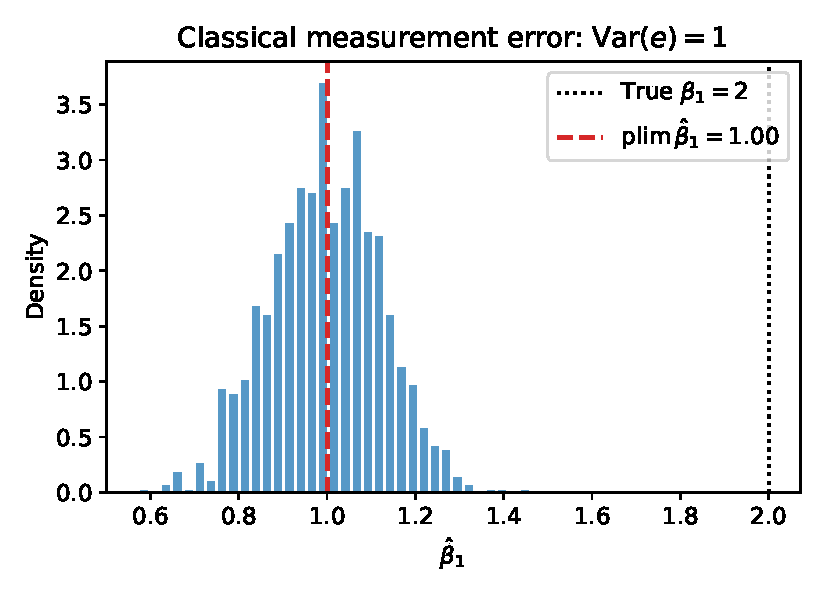
\includegraphics[origin=c,width=.72\textwidth]{Eksempler/Målefejl_hist e1 .pdf}

	$\hat\beta_1$ er centreret omkring $2\cdot 1/(1+1)=1$.
	\end{center}

\end{frame}

%%%%%%%%%%%%%%%%%%%%%%%%%%%%%%%%%%%%%%%%%%%%%%

%%%%%%%%%%%%%%%%%%%%%%%%%%%%%%%%%%%%%%%%%%%%%%
\begin{frame}
\frametitle{Monte Carlo: $\text{var}(e)=0.5$}

	\begin{center}
	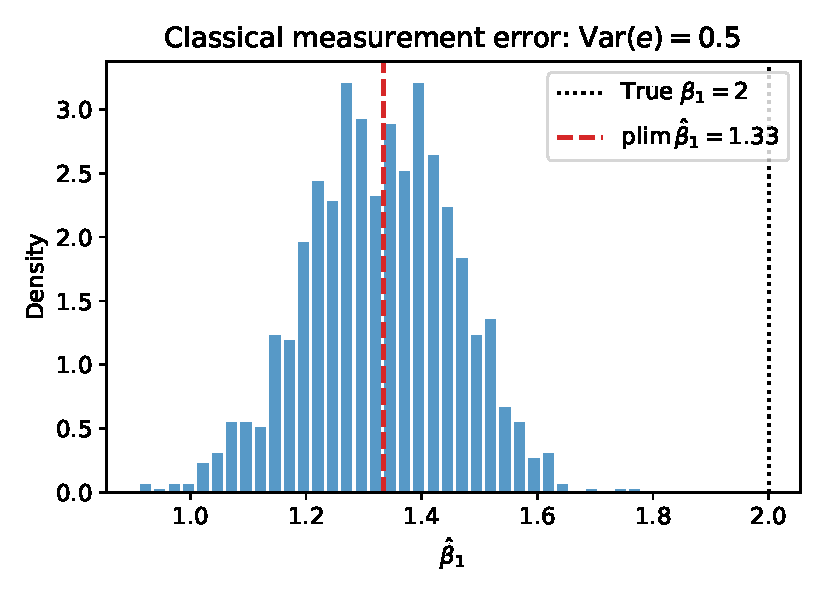
\includegraphics[origin=c,width=.72\textwidth]{Eksempler/Målefejl_hist e.5 .pdf}

	$\hat\beta_1$ er centreret omkring $2\cdot 1/(1+0.5)=4/3$.
	\end{center}

\end{frame}

%%%%%%%%%%%%%%%%%%%%%%%%%%%%%%%%%%%%%%%%%%%%%%

%%%%%%%%%%%%%%%%%%%%%%%%%%%%%%%%%%%%%%%%%%%%%%
\begin{frame}
\frametitle{Lad os se, om det passer!}
	\begin{center}
	\includegraphics[origin=c,width=.60\textwidth]{../06_simulation/figures/PythonLogo.jpg}
	\vspace{0.5em}
	\begin{itemize}
		\item \textbf{Jupyter Notebook:} \url{11_simulation_examples.ipynb}
		\item \textbf{Part 1:} Målefejl i den forklarende variabel
		\item Eksperimenter med attenuation bias og målefejlsvarians
	\end{itemize}
	\end{center}

\end{frame}
%%%%%%%%%%%%%%%%%%%%%%%%%%%%%%%%%%%%%%%%%%%%%%


\section[Dataproblemer]{Dataproblemer (W9.5)}


%%%%%%%%%%%%%%%%%%%%%%%%%%%%%%%%%%%%%%%%%%%%%%
\begin{frame}
\frametitle{Dataproblemer}

	Indtil nu har vi antaget, at \textbf{MLR.2} er opfyldt:
	\begin{itemize}
	\item MLR.2: Observationerne $(y_i,X_i)$ er uafhængige og identisk fordelte træk fra populationen.
	\end{itemize}
	Det er ikke altid tilfældet:
	\begin{itemize}
	\item Manglende observationer: tilfældigt eller ikke tilfældigt
	\item Dataudvælgelse: endogen eller eksogen udvælgelse
	\item Korrelerede fejlled (kun delvist dækket i Wooldridge)
	\end{itemize}
	Derudover skal vi snakke kort om problemer med
	\begin{itemize}
	\item Ekstreme observationer
	\end{itemize}
\end{frame}

%%%%%%%%%%%%%%%%%%%%%%%%%%%%%%%%%%%%%%%%%%%%%%


\subsection{Manglende observationer}


%%%%%%%%%%%%%%%%%%%%%%%%%%%%%%%%%%%%%%%%%%%%%%
\begin{frame}
\frametitle{Manglende observationer}

	Manglende observationer for en eller flere af variablene. 
	
	\textbf{Er det et problem?}
	\begin{itemize}
	\item Ud over at manglende observationer reducerer $n$.
	\end{itemize}
	Det er vigtigt at vide, hvorfor observationerne mangler.
	\begin{itemize}
	\item Lad $s=1$ betyde, at observationen indgår i stikprøven. Den centrale betingelse er
	\begin{equation*}
	E(u|X,s=1)=0.
	\end{equation*}
	\item Observationer må gerne mangle afhængigt af $X$, hvis denne betingelse fortsat holder.
	\end{itemize}
	Hvis $E(u|X,s=1)=0$, er OLS stadig \textbf{middelret og konsistent} i den observerede stikprøve.

\end{frame}

%%%%%%%%%%%%%%%%%%%%%%%%%%%%%%%%%%%%%%%%%%%%%%

%%%%%%%%%%%%%%%%%%%%%%%%%%%%%%%%%%%%%%%%%%%%%%
\begin{frame}
\frametitle{Hvornår er manglende observationer et problem?}

	Problemet opstår, når selektionen ændrer fejlleddets betingede middelværdi:
	\begin{equation*}
	E(u|X,s=1)\neq0.
	\end{equation*}
	Eksempler:
	\begin{itemize}
		\item Kun studerende, som er ekstraordinært glade eller sure, svarer på evalueringerne.
		\item Kun særligt dygtige lavtuddannede tager en IQ-test.
	\end{itemize}
	Det er altså ikke manglende observationer i sig selv, men \textbf{årsagen til, at de mangler}, som er afgørende.

\end{frame}

%%%%%%%%%%%%%%%%%%%%%%%%%%%%%%%%%%%%%%%%%%%%%%

%%%%%%%%%%%%%%%%%%%%%%%%%%%%%%%%%%%%%%%%%%%%%%
\begin{frame}
\frametitle{Opgave om manglende observationer}

	Vi skal se på, hvordan manglende observationer kan påvirke
	estimationen ved hjælp af et simulationseksperiment.
	
	Til simulationseksperimentet bruger vi, at 
	\begin{equation*}
	x\sim N(2,1),v\sim U(0,1),e\sim N(0,1),
	\end{equation*}
	Ud fra disse variable danner vi $u,y$ og $s$:
	\begin{align*}
	u &=e+2(v-0.5),  \\
	s &=1(v>0.2),     \\
	y &=1+x+u.
	\end{align*}
	Den sande model er $y=1+x+u$, men vi observerer kun $y$, når $s=1$.

\end{frame}

%%%%%%%%%%%%%%%%%%%%%%%%%%%%%%%%%%%%%%%%%%%%%%

%%%%%%%%%%%%%%%%%%%%%%%%%%%%%%%%%%%%%%%%%%%%%%
\begin{frame}
\frametitle{Opgave om manglende observationer}

	Vi bruger simulationen til at besvare følgende spørgsmål:

	\begin{itemize}
	\item Estimer modellen, hvor alle observationer bruges. Er OLS
	estimatoren for $\beta _{0}$ og $\beta _{1}$ middelret og konsistent?
	\medskip
	
	\item Estimer modellen, hvor der kun anvendes observationer 
	hvor $s=1$. Er OLS-estimatoren for $\beta _{0}$ og $\beta _{1}$
	middelret og konsistent?\medskip

	\item Hvilke aspekter af modellen er kritiske for resultaterne?
\end{itemize}

\end{frame}

%%%%%%%%%%%%%%%%%%%%%%%%%%%%%%%%%%%%%%%%%%%%%%

%%%%%%%%%%%%%%%%%%%%%%%%%%%%%%%%%%%%%%%%%%%%%%
\begin{frame}
\frametitle{Python-resultater}

	Monte Carlo med $n=500$ og 1.000 replikationer:
	\begin{center}
	\begin{tabular}{llcc}
	\toprule
	Stikprøve & Parameter & Sand værdi & Gns. estimat \\
	\midrule
	Alle observationer & $\beta_0$ & 1 & 1.000 \\
	                  & $\beta_1$ & 1 & 1.000 \\
	\addlinespace
	Kun $s=1$         & $\beta_0$ & 1 & 1.201 \\
	                  & $\beta_1$ & 1 & 1.000 \\
	\bottomrule
	\end{tabular}
	\end{center}

	\begin{itemize}
		\item Med alle observationer er begge estimatorer middelrette.
		\item Når kun $s=1$ observeres, ændres konstantleddet, men ikke hældningen.
	\end{itemize}

\end{frame}
%%%%%%%%%%%%%%%%%%%%%%%%%%%%%%%%%%%%%%%%%%%%%%

%%%%%%%%%%%%%%%%%%%%%%%%%%%%%%%%%%%%%%%%%%%%%%
\begin{frame}
\frametitle{Hvorfor ændres kun konstantleddet?}

	Når $s=1$, ved vi, at $v>0.2$. Derfor
	\begin{align*}
	E(v|s=1)&=0.6,\\
	E(u|s=1)&=E(e)+2\{E(v|s=1)-0.5\}=0.2.
	\end{align*}
	Da $x$ er uafhængig af selektionen,
	\begin{equation*}
	E(u|x,s=1)=0.2.
	\end{equation*}
	Regressionen i den observerede stikprøve er derfor
	\begin{equation*}
	y=1.2+x+\underbrace{(u-0.2)}_{\text{betinget middelværdi }0}.
	\end{equation*}
	Selektionen flytter konstantleddet, men ikke hældningen.

\end{frame}

%%%%%%%%%%%%%%%%%%%%%%%%%%%%%%%%%%%%%%%%%%%%%%

\subsection{Dataudvælgelse}


%%%%%%%%%%%%%%%%%%%%%%%%%%%%%%%%%%%%%%%%%%%%%%
\begin{frame}
\frametitle{Dataudvælgelse}

	Nogle gange er det os som økonometrikere, som udvælger data baseret på forskellige karakteristika (fx alder).
	
	Her skelner vi mellem
	\begin{itemize}

	\item \textbf{Eksogen dataudvælgelse:} baseret på forklarende variable.

	\item \textbf{Endogen dataudvælgelse:} baseret på den afhængige variabel.

	\item \textbf{Stratificerede data:} Oversampling af observationer med givne forklarende variable.
	
	\end{itemize}
	Nogle gange kommer vi til at udvælge data uden eksplicit at tænke over det.
	
	Som ved manglende observation, medfører ikke alle typer dataudvælgelse bias.

\end{frame}

%%%%%%%%%%%%%%%%%%%%%%%%%%%%%%%%%%%%%%%%%%%%%%

%%%%%%%%%%%%%%%%%%%%%%%%%%%%%%%%%%%%%%%%%%%%%%
\begin{frame}
\frametitle{Dataudvælgelse: Eksogen}

	Eksogen dataudvælgelse er baseret på en eller flere af de forklarende variable.
	\begin{itemize}
	\item Det er i udgangspunktet ikke et problem.
	
	\item Hvis $E(y|x)$ er den samme korrekt specificerede funktion i hele populationen,
			estimerer vi den samme populationskoefficient i forskellige intervaller af $x$.
			
	\item I så fald er OLS-estimatoren stadig middelret og konsistent.
	\end{itemize}	
	Hvis den funktionelle form er forkert, kan estimaterne ændre sig på tværs af stikprøver.

	\begin{itemize}	
	\item Det er ikke nødvendigvis et problem. Tværtimod kan det være nyttig information.
	\end{itemize}
	
	Stratifisering er et eksempel på eksogen dataudvælgelse.

\end{frame}

%%%%%%%%%%%%%%%%%%%%%%%%%%%%%%%%%%%%%%%%%%%%%%

%%%%%%%%%%%%%%%%%%%%%%%%%%%%%%%%%%%%%%%%%%%%%%
\begin{frame}
\frametitle{Hele stikprøven}

	\begin{center}
	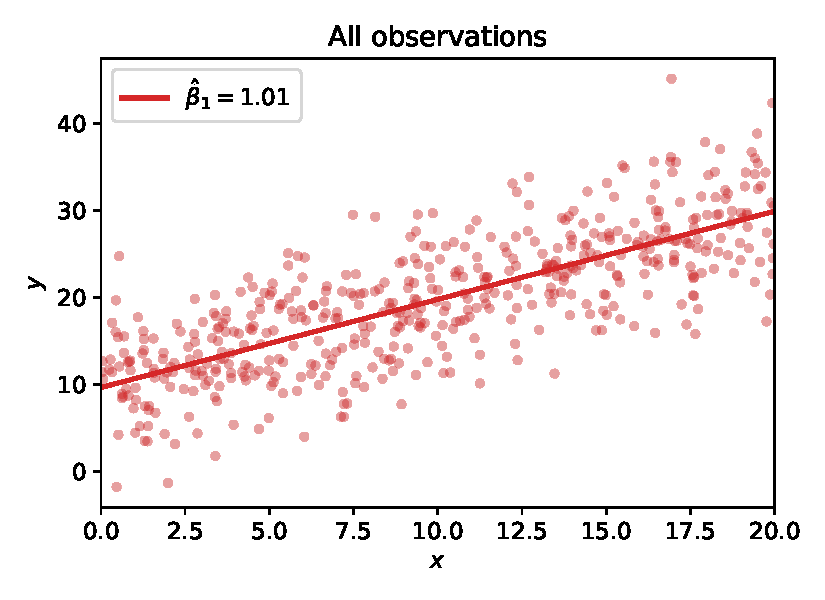
\includegraphics[origin=c,width=.70\textwidth]{Eksempler/Dataudvælgelse Alle.pdf}
	\end{center}

	Den estimerede linje beskriver den betingede sammenhæng i hele stikprøven.

\end{frame}

%%%%%%%%%%%%%%%%%%%%%%%%%%%%%%%%%%%%%%%%%%%%%%

%%%%%%%%%%%%%%%%%%%%%%%%%%%%%%%%%%%%%%%%%%%%%%
\begin{frame}
\frametitle{Eksogen udvælgelse: $x>5$}

	\begin{center}
	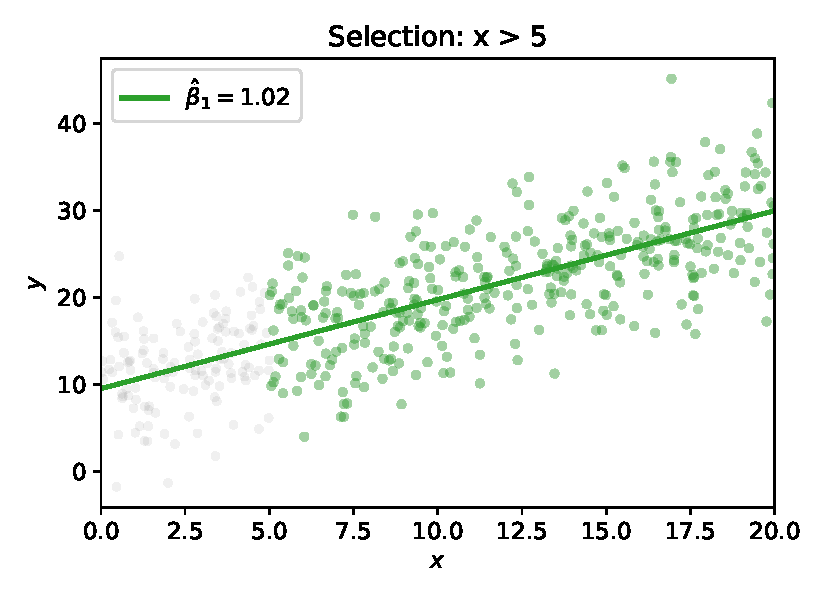
\includegraphics[origin=c,width=.70\textwidth]{Eksempler/Dataudvælgelse x5.pdf}
	\end{center}

	Ved en korrekt lineær model ændrer udvælgelse på $x$ ikke populationshældningen.

\end{frame}

%%%%%%%%%%%%%%%%%%%%%%%%%%%%%%%%%%%%%%%%%%%%%%

%%%%%%%%%%%%%%%%%%%%%%%%%%%%%%%%%%%%%%%%%%%%%%
\begin{frame}
\frametitle{Dataudvælgelse: Endogen}

	Endogen dataudvælgelse er baseret på den afhængige variabel - enten eksplicit eller implicit.

	\textbf{Eksempler}
	\begin{itemize}
	\item \textbf{Effekten af uddannelse på lønnen blandt lavtlønnede} \\
		   Uddannelse reducerer sandsynligheden for at være lavt lønnet. \\
		   Vi ender med en stikprøve af alle lavtuddannede og de dårligst lønnede højtuddannede.
		   \medskip
		   
		   \item \textbf{Effekten af uddannelse på timelønnen} \\
		   Vi observerer kun timelønnen for personer i arbejde. \\
		   Der kan være systematiske forskelle på personer i arbejde og personer, som ikke arbejder.
\end{itemize}

OLS-estimatoren vil generelt \textbf{ikke} være \textbf{middelret og konsistent}, fordi $E(u|X,s=1)\neq0$.

\end{frame}

%%%%%%%%%%%%%%%%%%%%%%%%%%%%%%%%%%%%%%%%%%%%%%

%%%%%%%%%%%%%%%%%%%%%%%%%%%%%%%%%%%%%%%%%%%%%%
\begin{frame}
\frametitle{Endogen udvælgelse: $y<15$}

	\begin{center}
	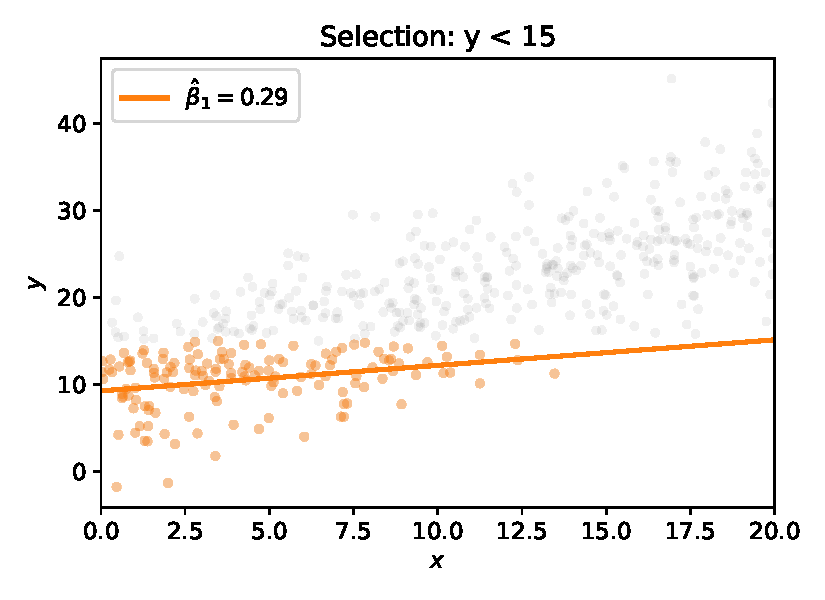
\includegraphics[origin=c,width=.70\textwidth]{Eksempler/Dataudvælgelse y15.pdf}
	\end{center}

	Udvælgelse på $y$ ændrer typisk $E(u|x,s=1)$ og dermed den estimerede hældning.

\end{frame}

%%%%%%%%%%%%%%%%%%%%%%%%%%%%%%%%%%%%%%%%%%%%%%

%%%%%%%%%%%%%%%%%%%%%%%%%%%%%%%%%%%%%%%%%%%%%%
\begin{frame}
\frametitle{Stikprøveudvælgelse: Hvad skal vi huske?}

	\begin{tabular}{p{0.29\textwidth}p{0.61\textwidth}}
	\toprule
	Selektionsmekanisme & Konsekvens \\
	\midrule
	Tilfældig eller kun baseret på inkluderede $X$
	& $E(u|X,s=1)=0$: Den oprindelige regressionsfunktion bevares. \\
	\addlinespace
	Baseret på $u$, men uafhængig af $X$
	& $E(u|X,s=1)$ kan være konstant: Konstantleddet ændres, mens hældningerne kan bevares. \\
	\addlinespace
	Baseret på både $X$ og $u$ --- eller direkte på $y$
	& $E(u|X,s=1)$ varierer typisk med $X$: Hældningerne bliver generelt biased. \\
	\bottomrule
	\end{tabular}

	\medskip
	Det afgørende er altså ikke blot, \emph{om} der er selektion, men hvordan selektionen ændrer $E(u|X,s=1)$.

\end{frame}

%%%%%%%%%%%%%%%%%%%%%%%%%%%%%%%%%%%%%%%%%%%%%%

%%%%%%%%%%%%%%%%%%%%%%%%%%%%%%%%%%%%%%%%%%%%%%
\begin{frame}
\frametitle{Lad os se, om det passer!}
	\begin{center}
	\includegraphics[origin=c,width=.57\textwidth]{../06_simulation/figures/PythonLogo.jpg}
	\vspace{0.4em}
	\begin{itemize}
		\item \textbf{Jupyter Notebook:} \url{11_simulation_examples.ipynb}
		\item \textbf{Part 2A:} Eksemplet fra slides
		\item \textbf{Part 2B:} Eksperimenter med forskellige selektionsmekanismer
	\end{itemize}
	\end{center}

\end{frame}
%%%%%%%%%%%%%%%%%%%%%%%%%%%%%%%%%%%%%%%%%%%%%%


\subsection{Ekstreme observationer}


%%%%%%%%%%%%%%%%%%%%%%%%%%%%%%%%%%%%%%%%%%%%%%
\begin{frame}
\frametitle{Ekstreme observationer}
	\small

 Ekstreme observationer er observationer, som skiller sig ud relativt til resten af stikprøven.

 Ekstreme observationer kan have stor betydning for OLS-estimaterne.
	\begin{itemize}
	\item En \textbf{outlier} har et stort residual.
	\item En observation med \textbf{høj leverage} har ekstreme værdier af de forklarende variable.
	\item En \textbf{indflydelsesrig observation} ændrer estimaterne mærkbart.
	\end{itemize}

 Hvorfor optræder der ekstreme observationer?

\begin{itemize}
\item Datafejl fx indtastningsfejl.
\item Databehandling, fx beregning af timeløn for personer med meget få timer.
\item Nogle observationer er reelt ekstreme, fx meget store virksomheder eller meget høje indkomster.
\end{itemize}

\end{frame}

%%%%%%%%%%%%%%%%%%%%%%%%%%%%%%%%%%%%%%%%%%%%%%

%%%%%%%%%%%%%%%%%%%%%%%%%%%%%%%%%%%%%%%%%%%%%%
\begin{frame}
\frametitle{Ekstreme observationer}

Hvad skal vi gøre med ekstreme observationer?

\begin{itemize}
\item Kontrollér først, om observationen skyldes en datafejl, og ret fejlen ved kilden.

\item Estimer med og uden de ekstreme observationer og se hvor stor forskel det gør.

\item Brug kun transformationer, fx logaritmer, når de er økonomisk og statistisk meningsfulde.

\item Der findes estimatorer, som er mindre følsomme over for ekstreme observationer.
\end{itemize}

\end{frame}

%%%%%%%%%%%%%%%%%%%%%%%%%%%%%%%%%%%%%%%%%%%%%%


\section*{Opsummering}


%%%%%%%%%%%%%%%%%%%%%%%%%%%%%%%%%%%%%%%%%%%%%%
\begin{frame}
\frametitle{Opsummering}

\begin{itemize}
\item En proxyvariabel kan reducere bias og i visse tilfælde genskabe middelretheden af OLS.
\medskip
\item Ikke-differentiel målefejl i den afhængige variabel giver typisk mindre præcise OLS-estimater.
\medskip
\item Klassisk målefejl i en enkelt forklarende variabel giver attenuation mod nul i simpel regression.
\medskip
\item Ved manglende observationer er den centrale betingelse $E(u|X,s=1)=0$.
\medskip
\item Dataudvælgelse på $X$, inkl. stratificering, er typisk uproblematisk for en korrekt specificeret regressionsmodel.
\medskip
\item Udvælgelse på $y$ medfører typisk $E(u|X,s=1)\neq0$ og dermed bias.

\end{itemize}

\end{frame}

%%%%%%%%%%%%%%%%%%%%%%%%%%%%%%%%%%%%%%%%%%%%%%



\end{document}























